\chapter{Deep Gated Multimodal Units} \label{chap:deepgmu}

In this chapter we propose a novel multimodal fusion approach to integrate information from multiple genomic sources. While most methods have solely relied on data fusion (early fusion) or decision level fusion (late fusion), our approach utilizes a series of cascading gated multimodal units to deeply connect the integration of data fusion and decision fusion.
%by a series of cascading layers

\section{Architecture}

The architecture of a dGMU first contains multiplicative gates designed to construct an intermediate representation of data from multiple modalities. The input modalities along with the intermediate representation are then fed to a decision network that fuses the predictions using an additional internal gate. This structure is illustrated in Figure \hl{BLANK}. 

\begin{figure}[h!]
    \centering
    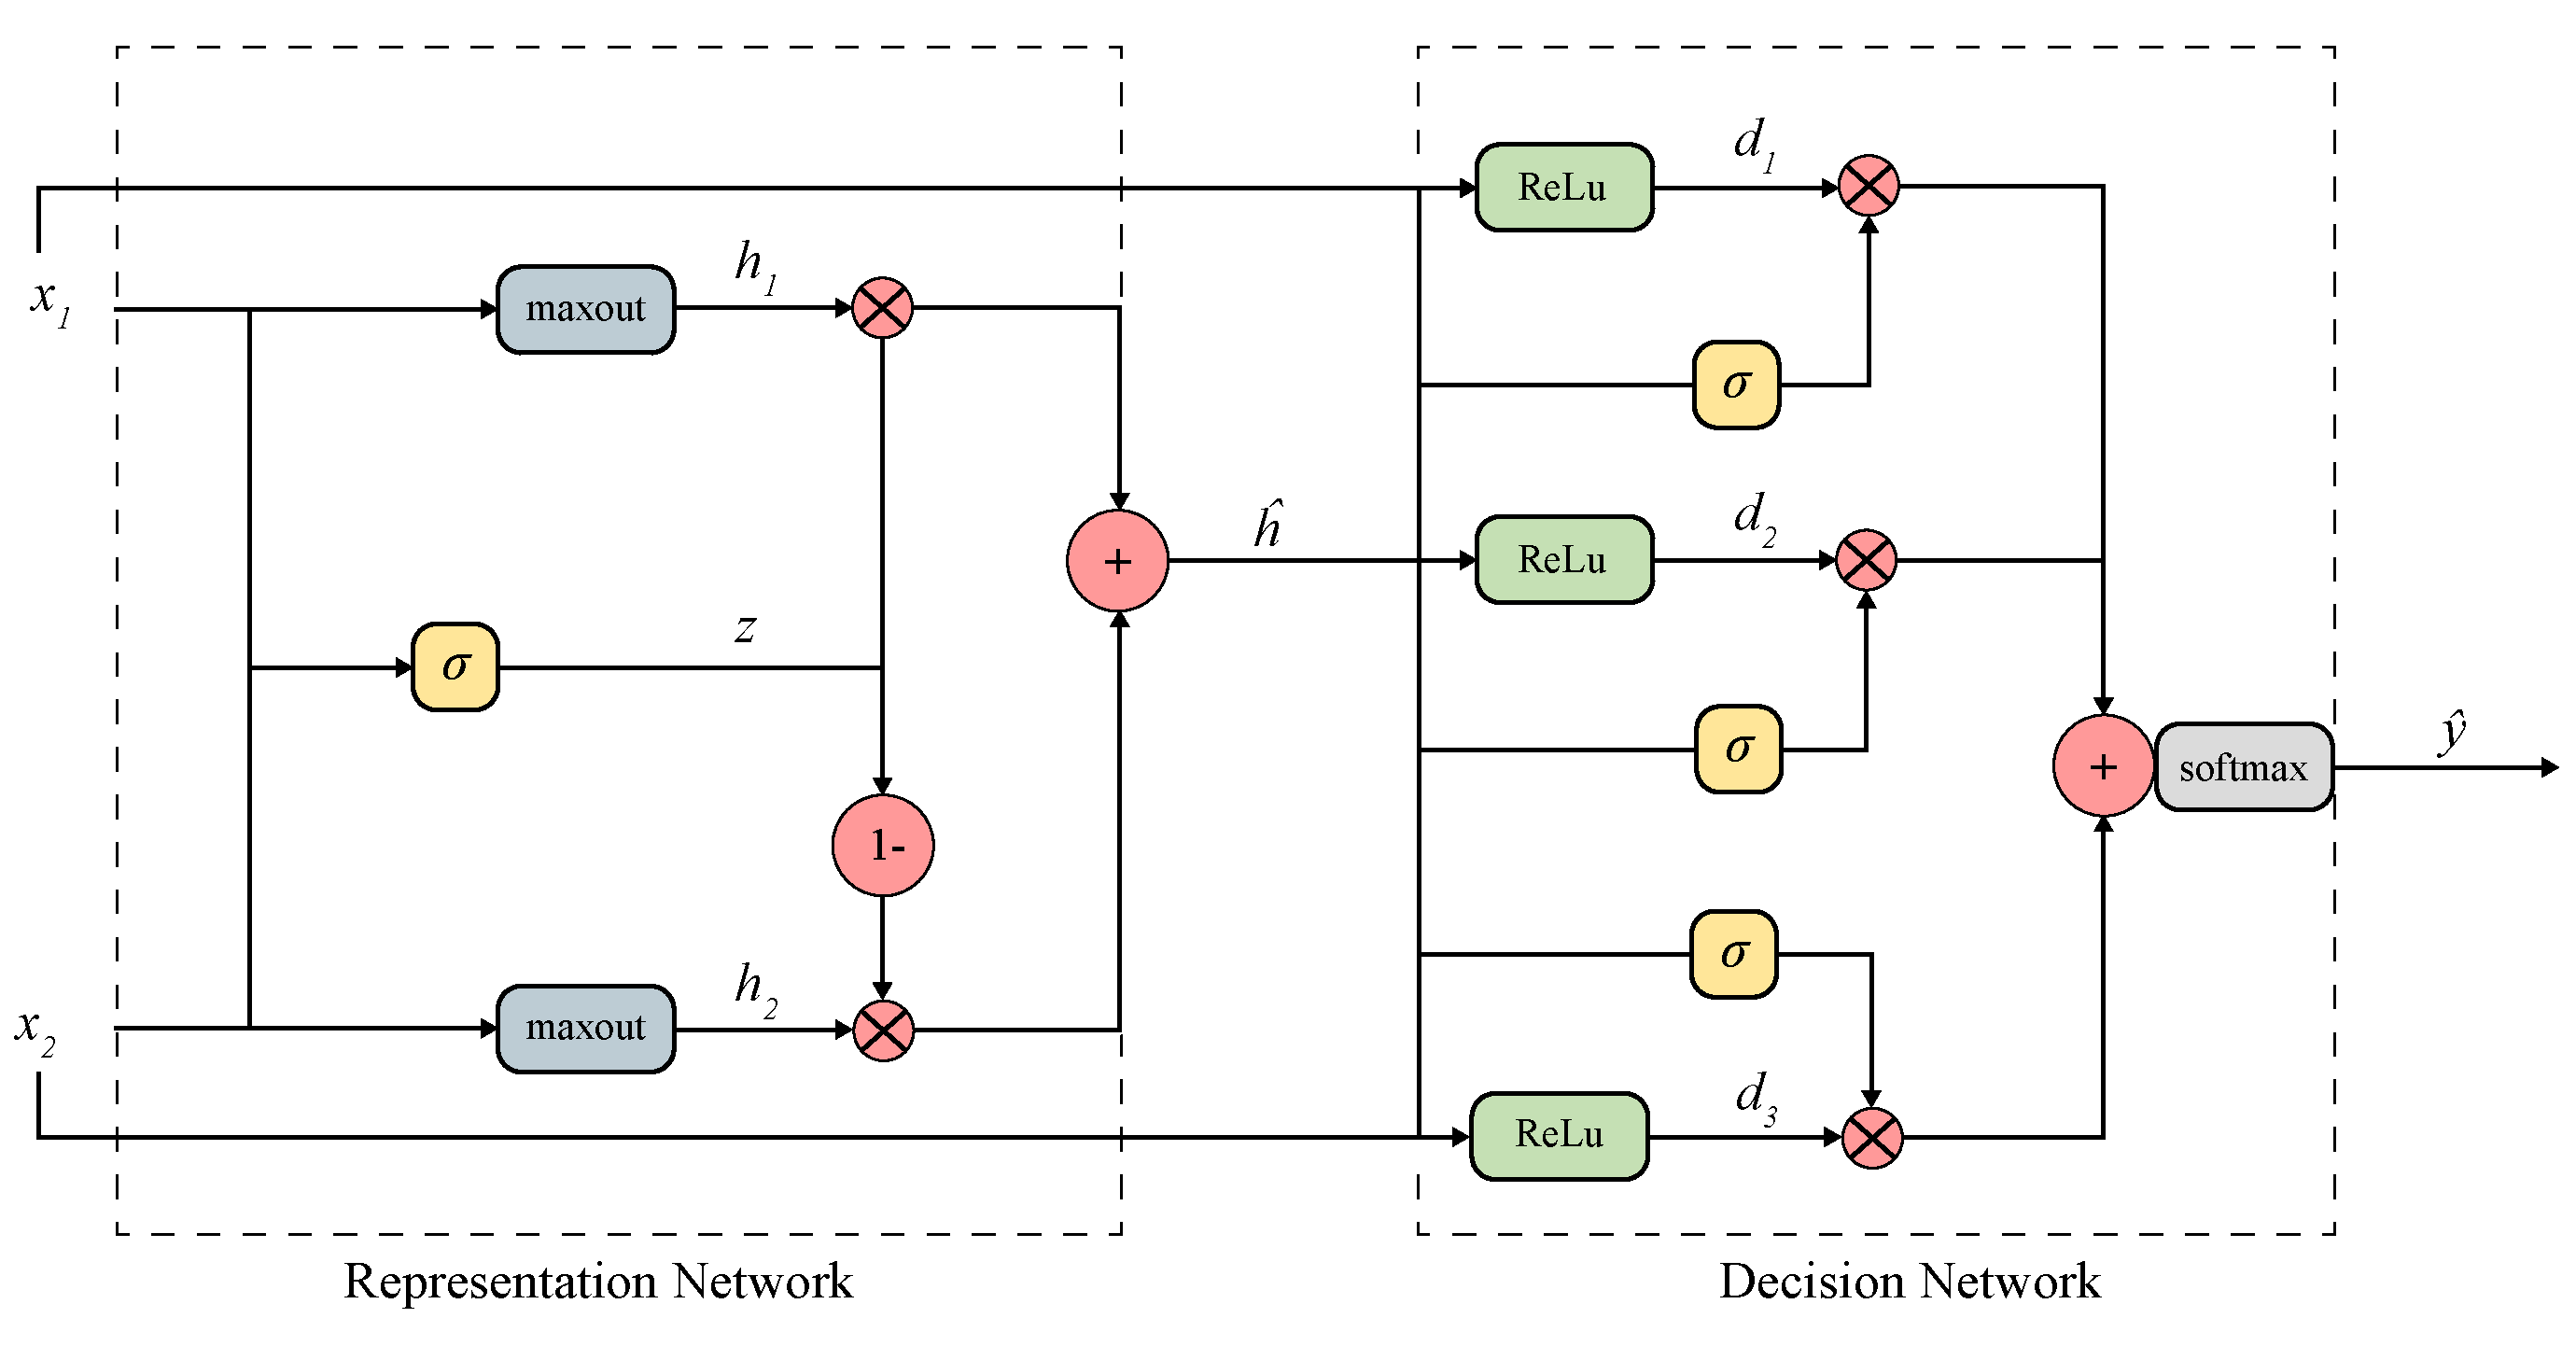
\includegraphics[width=\textwidth]{img/dGMU.png}
    \caption{Feedforward and Backpropagation Schematic.}
    \label{fig:backprop}
\end{figure}

The connection between the internal representation and decision networks are governed by the following equations:
%Internal gating neuron
%representation network
%decision network

\section{Training}
\section{Implementation}